\documentclass{article}

\usepackage{graphicx}
\usepackage{hyperref}
\usepackage{xcolor}

\title{Students Independent Study 1}
\author{Amangeldi Zhanserik}
\date{05 02 2005}

\begin{document}

\begin{titlepage}
    \centering

    \vspace*{1cm}

    \rule{\textwidth}{1pt}

    \vspace{2\baselineskip}

    {\huge  Cyber Security } \\

    \vspace{1\baselineskip}

    {\huge \textbf{ Lab 1: Install a Virtual Machine on a Personal Computer}}

    \vspace{2\baselineskip}

    \rule{\textwidth}{1pt}

    \vspace{1cm}

    \large

    \begin{flushleft}
        \begin{minipage}{.8\textwidth}
            \raggedright
            Fullname: Amangeldi Zhanserik \\
            ID: 22B030301 \\
            E-mail: {\normalsize \url{zha_amangeldi@kbtu.kz}} \\
            Date of submission: 05/02/2025 \\
            Class time: Thursday, 15:00--18:00 \\
        \end{minipage}%
    \end{flushleft}

    \vspace{2cm}

    
\includegraphics[width=.7\textwidth]{logo-kbtu.png}

    \vfill

    School of Information System and Engineering \\
    Kazakh-British Technical University \\
    Academic Year 2024-2025 \\
\end{titlepage}

\newpage

\section*{Part 1: Prepare a Host Computer for Virtualization}

In Part 1, I downloaded and installed desktop virtualization software, and also downloaded an image file that
was used to complete labs throughout the course.

\subsection*{Step 1: Download and install VirtualBox.}
I installed UTM instead of the suggested VMs, as it is better compatible with my MacBook.

\subsection*{Step 2: Download the Virtual Machine image file.}
I downloaded the virtual machine image file, and fortunately, it was perfectly compatible with UTM.

\section*{Part 2: Import the Virtual Machine into the VirtualBox Inventory}

In this part I started the VM image in UTM.

\subsection*{Step 1: Import the virtual machine files into VirtualBox.}

In this step will be some differentiation between my action and steps in laboratory work, because of I work in UTM.

\subsubsection*{A) Open the UTM and click the "+" or "Create a New Virtual Machine"}
\includegraphics[width=1\textwidth]{Part2/Step1/1.png}

\subsubsection*{B) Because of our downloaded image is existing VM, we can just "Open" this image. }
\includegraphics[width=1\textwidth]{Part2/Step1/2.png}

\subsubsection*{C) Choose the downloaded image and click "Open" }
\includegraphics[width=1\textwidth]{Part2/Step1/3.png}
\includegraphics[width=1\textwidth]{Part2/Step1/4.png}

\vspace{2\baselineskip}

After all this manipulation, I got working VM.

\newpage
\subsection*{Step 2: Start the CSE-LABVM virtual machine and log in.}

\subsubsection*{A) Choose the "Cybersecurity-LabVM-Workstation" named VM and click the play button in main menu of UTM}
\includegraphics[width=1\textwidth]{Part2/Step2/1.png}

\subsubsection*{B) Wait until the VM is loading and after appearing login menu, click the button "Log In"}
\includegraphics[width=1\textwidth]{Part2/Step2/2.png}

\newpage
\subsection*{Step 3: Familiarize yourself with "Cybersecurity-LabVM-Workstation".}

\includegraphics[width=1\textwidth]{Part2/Step2/3.png}

\vspace{1\baselineskip}

In this step I familiarized with every icons on Desktop. I have experience with Linux(Ubuntu, Debian and Fedora) and Wireshark, and It didn't get many time.

\vspace{1\baselineskip}

\textbf{Questions or Actions and Answers} 

\vspace{1\baselineskip}

\textbf{\colorbox{yellow}{Question 1: }} Open the terminal application. Type the ip address command at the prompt to determine the IP address of your virtual machine. What are the IP addresses assigned to your virtual machine? 

\textbf{Answer: }IP of interface "enp0s1" is 172.18.28.18, VM's IP

\includegraphics[width=0.5\textwidth]{Part2/Step2/4.png}

\newpage
\textbf{\colorbox{yellow}{Question 2: }}Locate and launch the web browser application. Can you navigate to your favorite search engine?

\textbf{Answer: } Yes, I was able. 

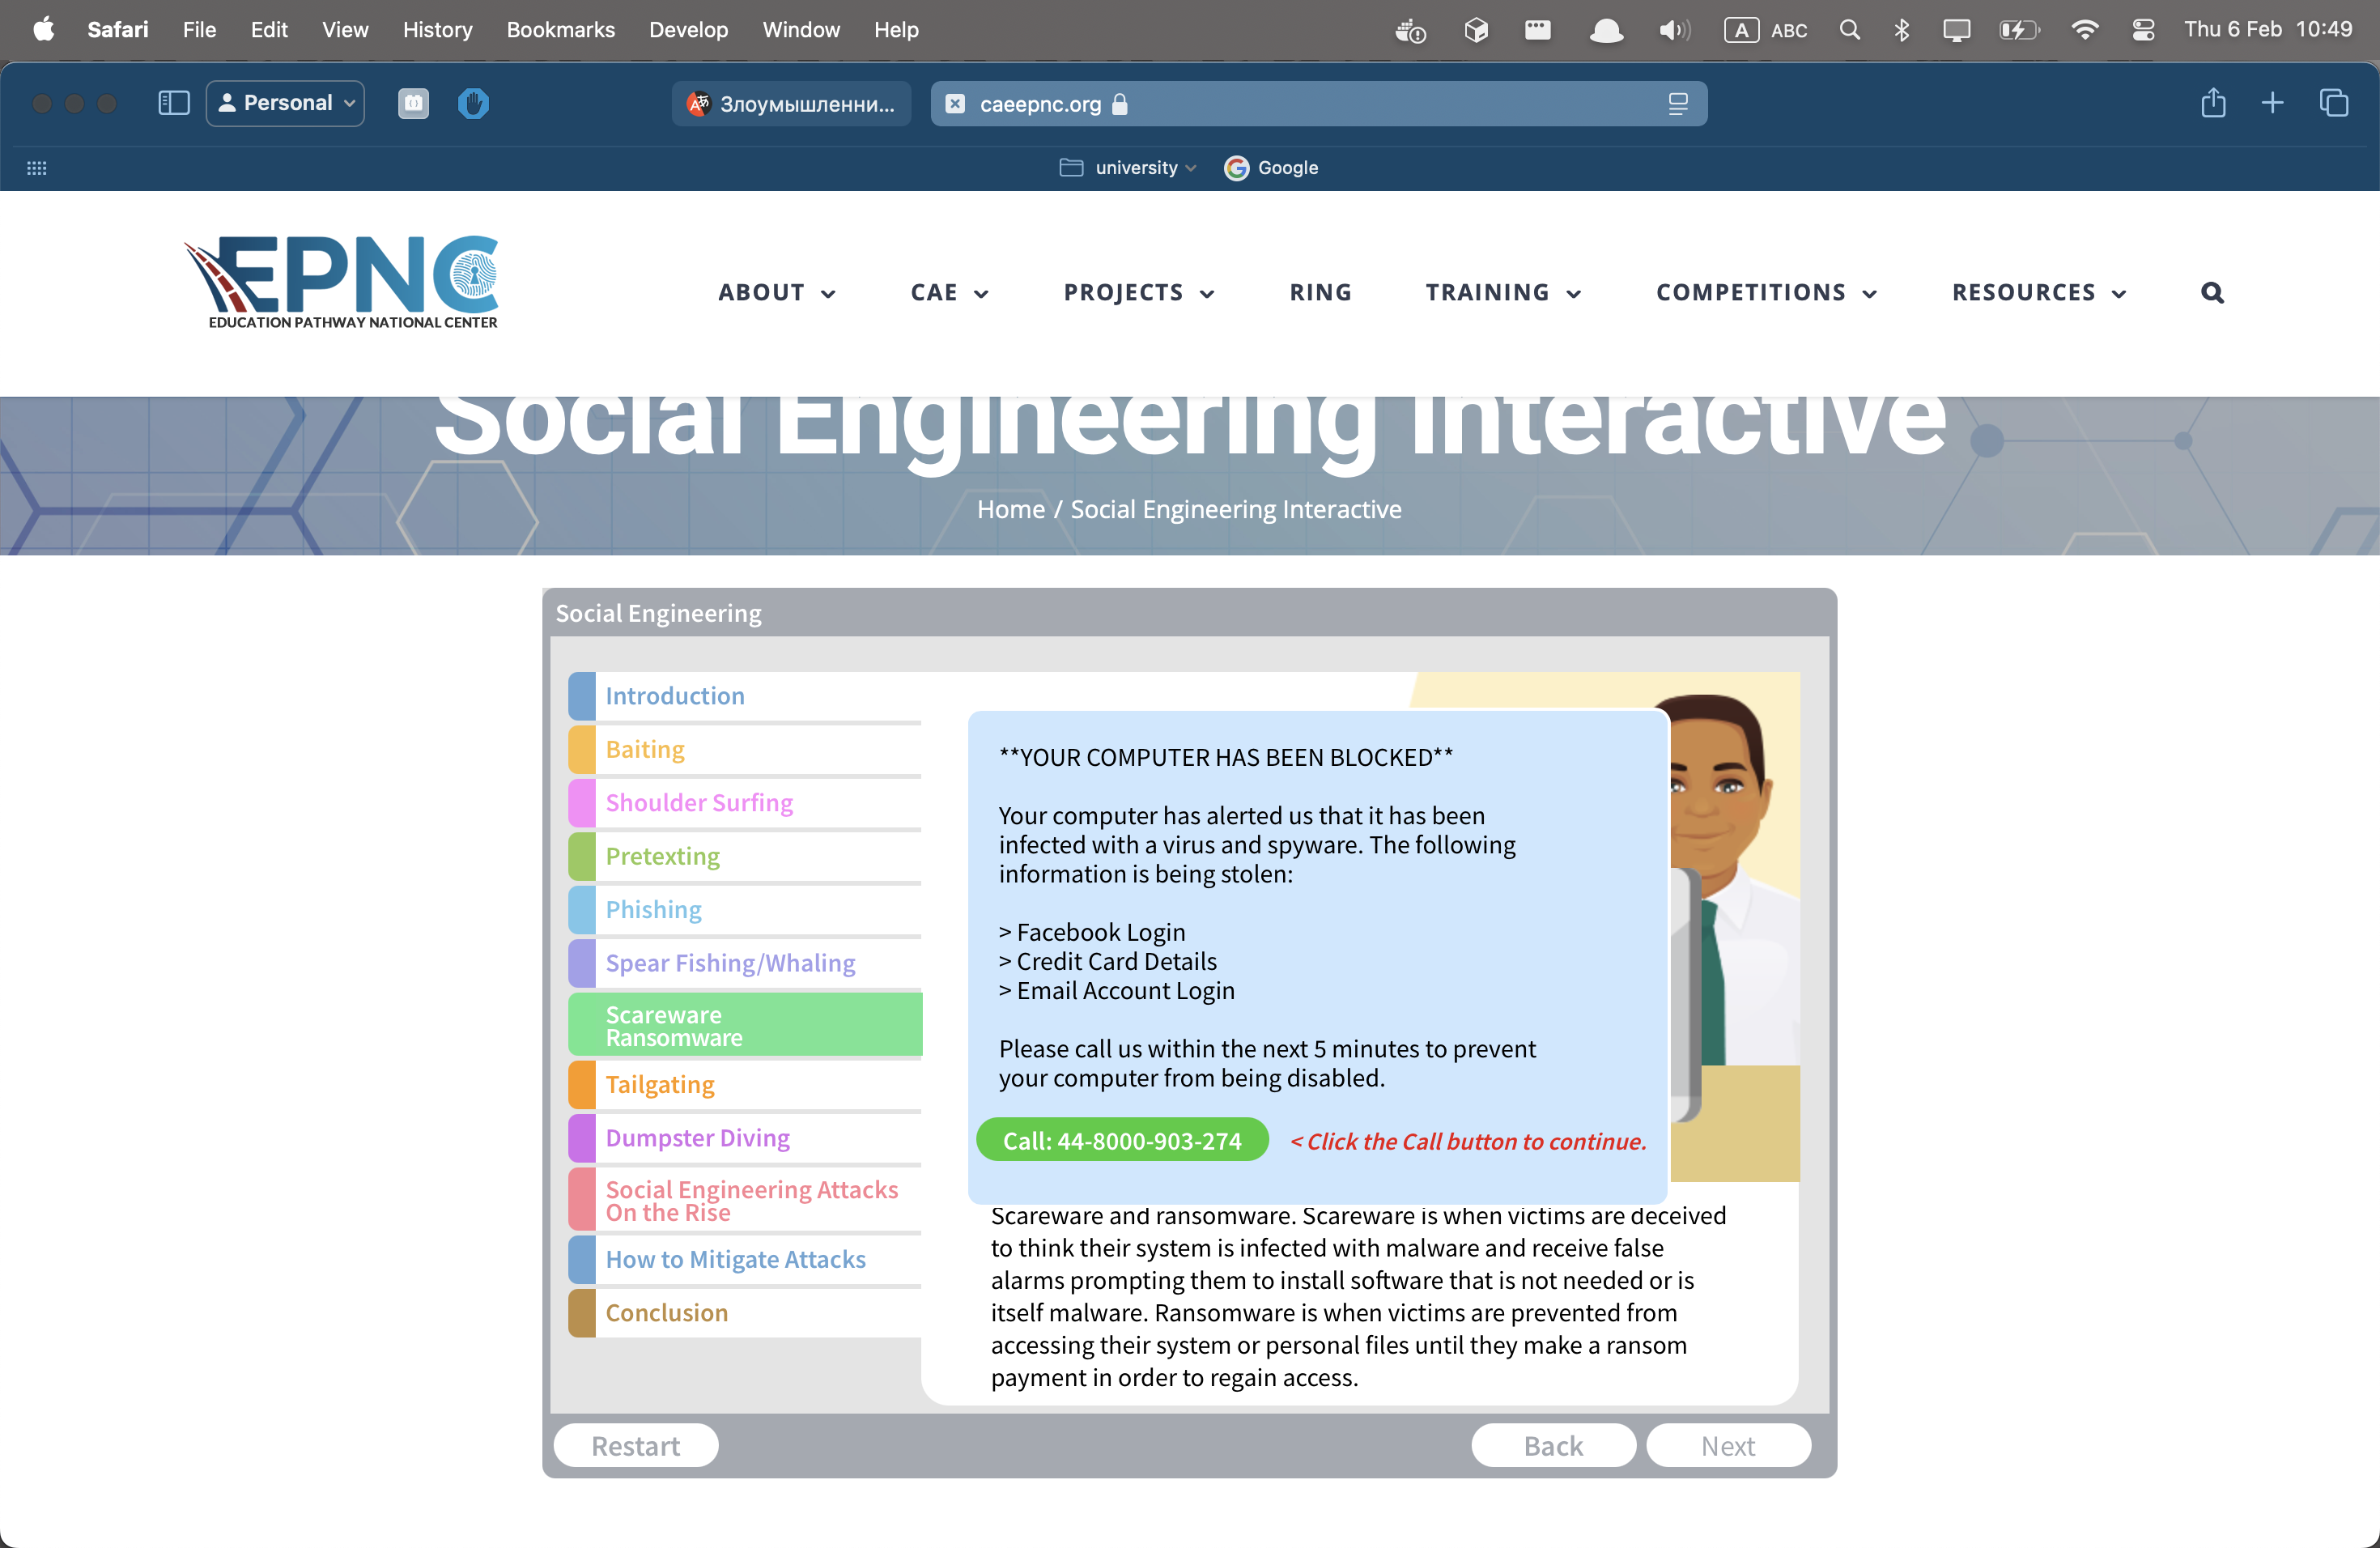
\includegraphics[width=0.5\textwidth]{Part2/Step2/5.png}

\subsection*{Step 4: Shutdown the Cybersecurity-LabVM-Workstation} 

\subsubsection*{A) Click the "File" button in the top left corner of the VM window and choose "Close" button.}

\includegraphics[width=1\textwidth]{Part2/Step4/1.png}

\newpage

\textbf{Questions or Actions and Answers} 

\vspace{1\baselineskip}

\textbf{\colorbox{yellow}{Question 1: }} What options are available? 

\vspace{1\baselineskip}

\textbf{Answer: } Because of I use UTM, I have only "OK" and "Cancel" buttons.

\vspace{1\baselineskip}

\includegraphics[width=0.5\textwidth]{Part2/Step4/2.png}

\subsection*{What about next steps?}
Because of now we use only one VM instead of two different, we can skip the next steps.

\section*{Reflection}
\colorbox{yellow}{What are the advantages and disadvantages of using a virtual machine?}

\vspace{1\baselineskip}

Using a virtual machine (VM) offers several advantages, such as the ability to run multiple operating systems on a single physical machine, which can save costs and resources. VMs provide a safe environment for testing and development, as they can be easily reset to a previous state if something goes wrong. They also enhance security by isolating different applications and services. However, there are some disadvantages, including potential performance overhead due to resource sharing between the host and guest systems. Additionally, VMs can be complex to manage and require significant storage and memory resources, which might not be feasible for all users.


\end{document}